\documentclass[a4paper]{article}
%\usepackage[swedish]{babel}
\usepackage[utf8]{inputenc}
\usepackage{a4wide}
\usepackage{appendix}
%vid problem, testa någon av följande:
%\usepackage[cp1252]{inputenc} under Windows
%\usepackage[applemac]{inputenc} under MacOS 9 eller tidigare
%\usepackage[latin1]{inputenc} under MacOS X

%\usepackage{svg}
\usepackage[T1]{fontenc}
\usepackage[pdftex]{graphicx}

%\LaTeX\ är kul. Den senaste stora versionen heter \LaTeX2e och släpptes 1994~\cite{lamport94}.
%\begin{equation}
%a^2+b^2=c^2
%\label{eq:Pythagoras}
%\end{equation}
%För Pythagoras ekvation, se Ekvation~\ref{eq:Pythagoras}.

%\begin{figure}[h]
%\centering
%
\includegraphics[scale=0.9, angle=20]{bth_logo.jpg}
%
\includegraphics[scale=0.8, angle=40]{bth_logo.jpg}
%
\includegraphics[scale=0.7, angle=60]{bth_logo.jpg}
%\caption{Roterade BTH-logotyper}
%\label{fig:Logo}
%\end{figure}

%Bilder kan roteras med hjälp av en dator, se exempel i Figur~\ref{fig:Logo}.

\title{\Huge A* Pathfinding Acceleration with use of Auto-Generated Waypoints for Grid Traversal}
\author{Fredrik Olsson, Magnus Nyqvst}
\date{\today} 

\begin{document}
\pagenumbering{gobble}
\maketitle
\newpage
\thispagestyle{empty}
\paragraph{Abstract--}
Sammanfattar rapporten
Varför är vår rapport värd att läsa?
Syfte, metod
Viktiga resultat och slutsatser Nyckelord
“Tänk på att detta skall kunna läsas fristående”

\tableofcontents
\listoffigures
\newpage
\pagenumbering{arabic}
\twocolumn
\section{Introduction}
This is introduction lol \newline
Syfte \newline
Frågeställning \newline
Hypoteser \newline
Avgränsningar

\section{Background}
Stort spel \newline
Bakgrundsfakta (Definitioner som du använder dig av senare) \newline
Saker som läsaren behöver veta för att förstå din rapport \newline
Vad har gjorts tidigare?

\section{Related work}
Informationssökning \newline
Urval av litteratur - skriv inte om allt utan det viktigaste för din rapport

\section{Method}
Hur vi autogenerar (mycket referens till research articles) \newline
Vad har du gjort? \newline
Vilka metoder har du använt? \newline
Vad har du kommit fram till? \newline
Var noggrann och utförlig så att det går följa vad du gjort? \newline
Motivera om du antar något \newline
Diskutera begränsningar

\makeatletter
\setlength{\@fptop}{0pt}
\makeatother

\begin{figure}[t!]
\centering
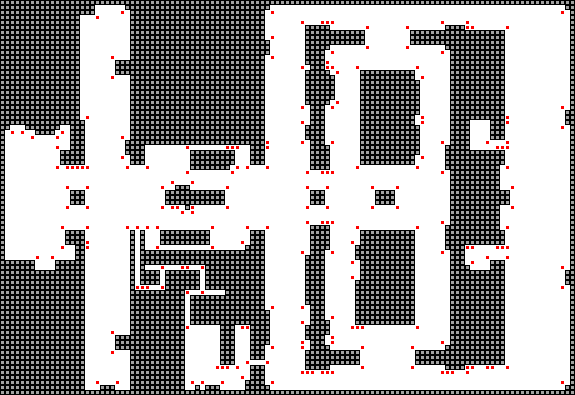
\includegraphics[width=0.5\textwidth,height=\textheight,keepaspectratio]{Data/Edgy.png}
\caption{Map Edgy}
9085 tiles, 4226 blocked (46.5\%). 214 waypoints with 2228 connections
\label{fig:Edgy}
\end{figure}

\begin{figure}[t!]
\centering
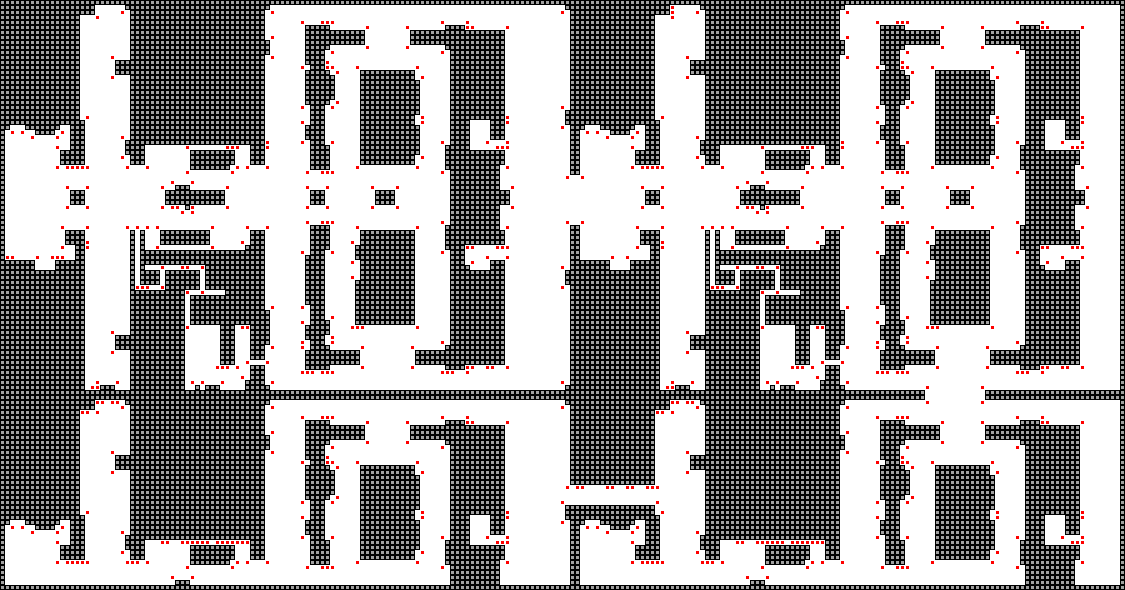
\includegraphics[width=0.5\textwidth,height=\textheight,keepaspectratio]{Data/Edgy2.png}
\caption{Map Edgy2}
26550 tiles, 12854 blocked (48.4\%). 658 waypoints with 6458 connections
\label{fig:Edgy2}
\end{figure}

\begin{figure}[t!]
\centering
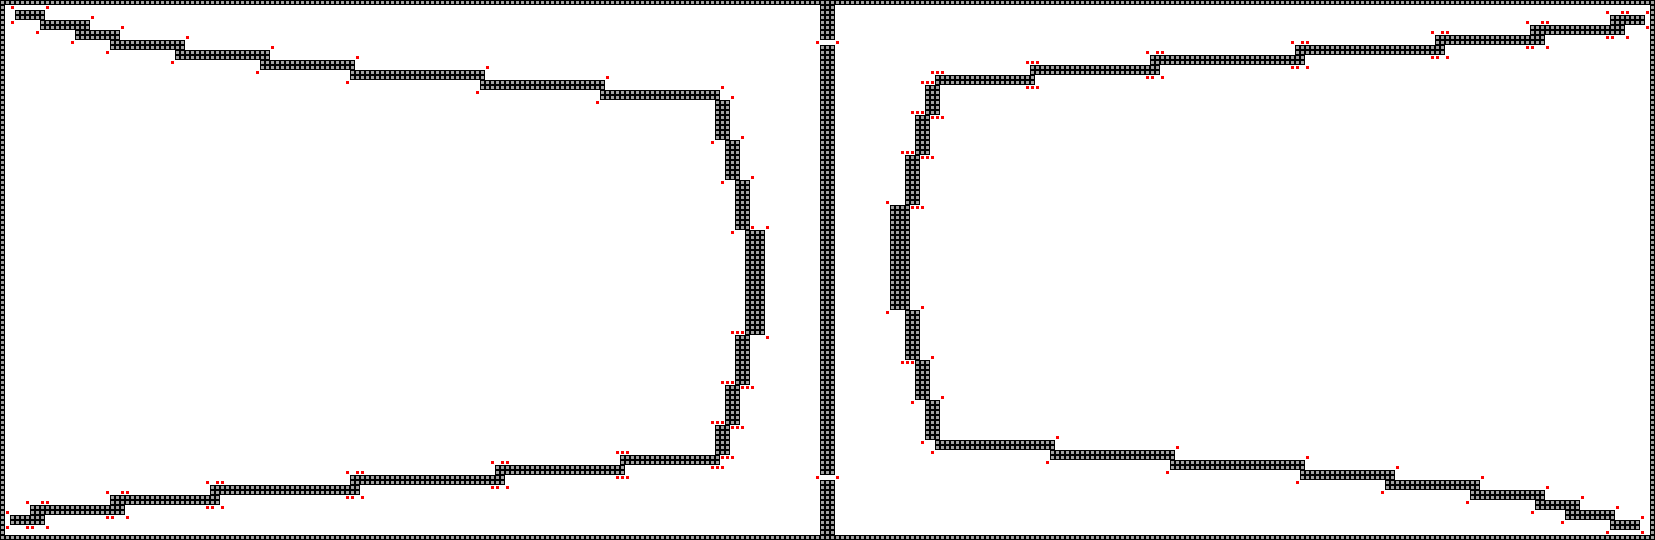
\includegraphics[width=0.5\textwidth,height=\textheight,keepaspectratio]{Data/UMAP2.png}
\caption{Map UMAP2}
35748 tiles, 2890 blocked (8\%). 179 waypoints with 2038 connections
\label{fig:UMAP2}
\end{figure}





\section{Result}
Every experiment done has shown a P value below 0.5. The results show that the the waypoints prove to be helpful for the A* algorithm in form of speed, which is the initial purpose of this research, whith an exception of the smallest map Edgy.
On this map, the based on the results, it dosnt matter what heuristics 


\section{Discussion}
On smaller maps with a lot of waypoint connections, raw A* is quicker than with our generation of waypoints. But when the map starts to scale, waypoints are significantly better than just A* by itself.

\newpage
\begin{thebibliography}{9}

\bibitem{lamport94}
  Leslie Lamport,
  \textit{\LaTeX: a document preparation system},
  Addison Wesley, Massachusetts,
  2nd edition,
  1994.

\end{thebibliography}

\end{document}
